\subsection{Komponen \textit{Resource Controller}}

Komponen ini terdiri dari sebuah kelas. Seperti namanya, kelas ini berfungsi untuk menggunakan \textit{Kubernetes Client API} untuk mengubah alokasi sumber daya. Kelas ini diimplementasikan dengan sistem antrian, sehingga jika sejumlah rule aktif secara bersamaan, maka akan dijalankan secara berurutan. Terdapat sebuah fungsi \textit{tick} yang akan berfungsi untuk mengeksekusi antrian. Spesifikasi kelas ini dapat dilihat pada gambar \ref{fig:rc-spek}.

\begin{figure}[h]
    \centering
    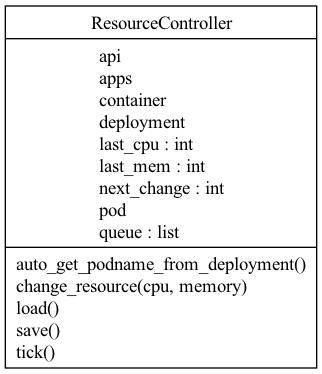
\includegraphics[width=0.4\textwidth]{chapter-4/rc.png}
    \caption{Spesifikasi Kelas Penyusun Komponen \textit{Resource Controller}}
    \label{fig:rc-spek}
\end{figure}

% TODO CONTOH SISTEM ANTRIAN